\chapter{Set-membership identification}    % For a new chapter (works in book and report class)

Set-membership approach is an alternative to the classical, statistical identification approach. Least-Square method is one possible example of statistical estimation algorithms in the context of estimation.\\

\subsubsection{Main ingredients}

We consider a discrete-time system described in the following parametrized regression form:\\
\begin{equation}
y(k) = f(y(k-1), y(k-2), \cdots, y(k-n), u(k), u(k-1), \cdots, u(k-m), \theta_1, \theta_2, \cdots, \theta_{n+m+1})
\end{equation}

where \(m\leq n\)\\
A-priori information on the system:
\begin{itemize}
    \item \(n\) and \(m\) are known
    \item \(f \in \mathbb{F}\) where \(\mathbb{F}\) is the class of model selected on the basis of our physical insight. 
\end{itemize}


A-priori information on the noise, the main difference with respect to the previous discussion.
\begin{itemize}
    \item the noise structure is known, i.e. the way the way uncertainty affects the input-output data)
    \item the noise is assumed to belong to konwn bounded set \(\mathbb{B}\).
\end{itemize}

When the consistency property of LS was discussed, and in general statistical approach to system identification, the typicall assumption on the noise is that statistical distribution of the noise sequence, or the value of some moments of inertia of the noise is known, such as variance. Here, the assumption is that the noise sequence \(\eta\) belongs to a bounded \(\mathbb{B}\). Remember that assumption two of the consistency property was the crucial one, so a change of perspective is adopted on the second assumption, where we deal with the following problem:

\textbf{Set-membership identification of LTI system} under the assumption that the uncertainty affecting the data can be modelled as an equation error \(e(k)\), which is exactly assumption \(1\) considered for the consistency theorem.\\
\[
\begin{aligned}
\tilde{y}(k) = & -\theta_1 \tilde{y}(k - 1) - \theta_2 \tilde{y}(k - 2) - \cdots - \tilde{y}(k - n) \\[1ex]
               & + \theta_{n+1} \tilde{u}(k) + \theta_{n+2} \tilde{u}(k - 1) + \cdots + \theta_{n+m+1} \tilde{u}(k - m) + \mathbf{e(k)} \\[2ex]
\end{aligned}
\]
where,
\[
\begin{aligned}
e(k) \in \mathbb{B}e = \left\{ \bar{e} = [e(1), e(2), \cdots, e(H)]^T \right\} : \left| e(k) \right| \leq \Delta e, \forall k
\end{aligned}
\]
where  \(\Delta e \) is a given real bounded constant.

\begin{factbox}[]
In set-membership, we always have unknown and bounded assumption about the magnitude of noise.\\

The bound is considered a conservative bound.

\end{factbox}
\subsubsection{Error-in-Variable setting}
Let's assume that the data are actually collected from a real experiment, which is EIV setup. The block-diagram representation of this a-priori information is as follows.

\begin{center}
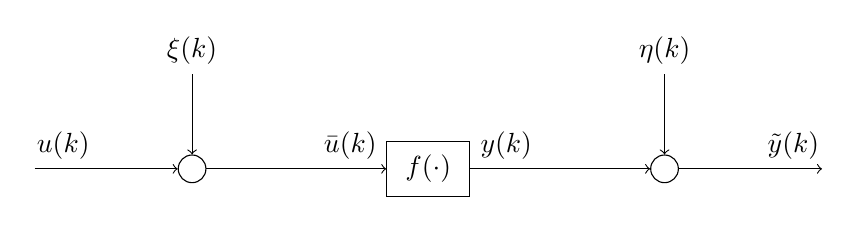
\begin{tikzpicture}[auto, node distance=2cm]

    % Block styles
    \tikzstyle{block} = [draw, rectangle, minimum height=2em, minimum width=3em]
    \tikzstyle{sum} = [draw, circle, inner sep=0pt, minimum size=1em]
    \tikzstyle{input} = [coordinate]
    \tikzstyle{output} = [coordinate]

    % Nodes
    \node [input] (input) {};
    \node [sum, right of=input, node distance=2cm] (sum1) {};
    \node [block, right of=sum1, node distance=3cm] (system) {$f(\cdot)$};
    \node [sum, right of=system, node distance=3cm] (sum2) {};
    \node [output, right of=sum2, node distance=2cm] (output) {};

    % Connections
    \draw [->] (input) -- node[pos=0.2] {$u(k)$} (sum1);
    \draw [->] (sum1) -- node[pos=0.8] {$\bar{u}(k)$} (system);
    \draw [->] (system) -- node[pos=0.2] {$y(k)$} (sum2);
    \draw [->] (sum2) -- node[pos=0.8] {$\tilde{y}(k)$} (output);
    
    % Noise terms
    \node [above of=sum1, node distance=1.5cm] (xi) {$\xi(k)$};
    \draw [->] (xi) -- (sum1);
    
    \node [above of=sum2, node distance=1.5cm] (eta) {$\eta(k)$};
    \draw [->] (eta) -- (sum2);

\end{tikzpicture}
\end{center}

\textit{Errors-in-variables} (EIV) problems refer to the most general case where both the input and the output collected samples are affected by noise.

\[
\xi = [\xi(1), \dots, \xi(H)] \in \mathcal{B}_{\xi}
\]
\[
\eta = [\eta(1), \dots, \eta(H)] \in \mathcal{B}_{\eta}
\]

$\mathcal{B}_{\xi}$ and $\mathcal{B}_{\eta}$ are bounded sets described by \textbf{\textit{polynomial constraints}.}

Most common case:
\[
\mathcal{B}_{\eta} = \left\{\eta : |\eta(k)| \leq \Delta_{\eta}\right\}, \quad \mathcal{B}_{\xi} = \left\{\xi : |\xi(k)| \leq \Delta_{\xi}\right\}
\]
Here, $f(.)$ belogn to a class of function $\mathbb{F}$, which is the a-priori assumption on the system.\\

Considering this a-priori information about the structure of the course, and a-priori information about the system, which is LTI second-order system. The noises can be reformulated as \textbf{Error-in-Equation}, which is the same as the first assumption of the consistency property of Least Square.


\[
\begin{array}{l}
\tilde{y}(k)= -\theta_1 \tilde{y}(k - 1) - \theta_2 \tilde{y}(k - 2) + \theta_3 \tilde{u}(k) + \theta_4 \tilde{u}(k - 1) + \theta_5 \tilde{u}(k - 2) \\[1ex]
\textcolor{red}{\fbox{\textcolor{black}{$+ \theta_1\eta(k-1) + \theta_2\eta(k-2) - \theta_3\tilde{u}(k) - \theta_4\tilde{u}(k-1) - \theta_5\tilde{u}(k-2) + \eta(k) $}}} =: + e(k) \\
\end{array}
\]

Up till now, nothing is changes, we now that statistically this kind of error is not i.i.d. The difference in is regarding the second assumption about the noise, \(e(k)\), which is the boundedness of the noise:

\[\left| e(k)\right| \leq \Delta e \forall k = 1, 2, ..., N\]

Provided that we find a way to compute the bound \(\Delta e \), on \(\left| e(k)\right|\), the identification problem can be correctly formulated in terms of \textbf{Equation-Error} structure in Set-membership framework. \textbf{However, Computing \(\Delta e \) is not an easy task}. Since it cannot be done without any assumption about \(\theta_i\), since they are to be identified.

\subsubsection{Set-membership formulation of the problem identifying a second order LTI system assuming an Equation-Error structure for the uncertainty}
Main ingredients:
\begin{enumerate}
\item \textbf{a-priori information }about the system, second order LTI, and the noise, Equation-Error structure and boundedness.
\item\textbf{ a-posteriori information} are experimentally collected input-output data samples.
\end{enumerate}
Now, here, we have the concept of \textit{Feasability Parameter Set}.

\subsubsection{Feasability parameter set}
The feasability parameter set \(\mathbb{D}_\theta\) is the set of all the values of the parameter vector \(\theta = \left[ \theta_1 \theta_2 \cdots \theta_p \right]^T \in \mathbb{R}^p\), which are consistent with all the avialable information on the system and the noise, and all he collected data.\\
To better understand the meaning of FPS, \(\mathbb{D}_\theta\), let's assume that we are collecting data according to the following\textbf{ Output-Error} setup:\\

\begin{center}    % Block styles
\begin{tikzpicture}[auto, node distance=2cm]

    \tikzstyle{block} = [draw, rectangle, minimum height=2em, minimum width=3em]
    \tikzstyle{sum} = [draw, circle, inner sep=0pt, minimum size=1em]
    \tikzstyle{input} = [coordinate]
    \tikzstyle{output} = [coordinate]

    % Nodes
    \node [input] (input) {};
    \node [block, right of=input, node distance=3cm] (system) {$f(\cdot)$};
    \node [sum, right of=system, node distance=3cm] (sum2) {};
    \node [output, right of=sum2, node distance=2cm] (output) {};

    % Connections
    \draw [->] (input) -- node[pos=0.5] {$u(k)$} (system);
    \draw [->] (system) -- node[pos=0.2] {$y(k)$} (sum2);
    \draw [->] (sum2) -- node[pos=0.8] {$\tilde{y}(k)$} (output);
    
    % Noise terms at the output
    \node [above of=sum2, node distance=1.5cm] (eta) {$\eta(k)$};
    \draw [->] (eta) -- (sum2);
\end{tikzpicture}
\end{center}\vspace{1cm}


Since, we have the following form of noise:\\
\[y(k) = \tilde{y} - \eta(k)\]
and we know that \(\eta\) is bounded. we can obtain the following relationship about the \(y(k)\), being that the real \(y(.)\) signal is enveloped in the following fashion:\\
\[
\tilde{y}(k) - \eta{k} \leq y(k) \leq \tilde{y}(k) + \eta{k}
\]

\begin{figure}[htbp]  % "h" for here, "t" for top, "b" for bottom, "p" for float page
    \centering
    \includegraphics[width=0.75\textwidth]{images/FPS_time_domain.jpg}
    \caption{The bounds for \(y\) encompass all the elements of the \(\theta\) vector, leading to a relation for \(y\) such that its graph is bounded between the represented bounds.}
    \label{fig:FPS_time_domain}
\end{figure}

\begin{factbox}[Professor's Quotes]
In the statistical identification, assuming probabilistic characteristics for the noise, instead of having bounded interval around each single sample of the output that we collect, we have a normal distribution around each single point. Therefore, a correct formulation of the identification, again, in that context, lead to a set of models, but this time instead of having a bounded set of possible models solving the problem, we obtain a set that is statistically described, where each models have a certain probability of being the correct model.
\end{factbox}

Now, let's try to define mathematically, the FPS \(\mathbb{D}_\theta\)
\[
\begin{aligned}
\mathbb{D}_\theta = \{
\theta = \left[\theta_1 \, \theta_2 \, \cdots \, \theta_p \right]^T \in \mathbb{R}^p \, | \, 
\tilde{y}(k) = & -\theta_1 \tilde{y}(k - 1) - \theta_2 \tilde{y}(k - 2) + \theta_3 \tilde{u}(k) + \theta_4 \tilde{u}(k - 1) \\
& + \theta_5 \tilde{u}(k - 2) + e(k) \, | \, \forall k > 3 \,,\, |e(k)|\leq \Delta e
\}
\end{aligned}
\]
However, this mathematical description is not correct, since here we define FPS as a subset of \textbf{parameter space}, \(\mathbb{R}^p\), but the description of the unknown error is not in the parameter space. How can we reformulate? Although we don't know \(e\), we know that this unknown error is bounded by \(\Delta e\), so how can we exploit this information?

\[
\begin{array}{l}
\mathbb{D}_\theta = \{
\theta \in \mathbb{R}^p \, | \, 
e(k) = \tilde{y}(k) + \theta_1 \tilde{y}(k - 1) + \theta_2 \tilde{y}(k - 2) 
- \theta_3 \tilde{u}(k) - \theta_4 \tilde{u}(k - 1) - \theta_5 \tilde{u}(k - 2), \\
\forall k > 3 \,,\, |e(k)| \leq \Delta e
\}
\end{array}
\]
\[
\Rightarrow
\begin{array}{l}
\mathbb{D}_\theta = \{
\theta \in \mathbb{R}^p \, : \, 
|\tilde{y}(k) + \theta_1 \tilde{y}(k - 1) + \theta_2 \tilde{y}(k - 2) 
- \theta_3 \tilde{u}(k) - \theta_4 \tilde{u}(k - 1) - \theta_5 \tilde{u}(k - 2)|\leq \Delta e, \\ \forall k > 3
\}
\end{array}
\]
Now, we have obtained \textbf{an implicit description} of the set of \textbf{all the feasible solutions to our identification problem}, in terms of a set of inquality constraints only involving \(\theta\). \(\mathbb{D}_\theta\) is now clearly a subset of the parameter space \(\mathbb{R}^p\).

Graphical representation of \(\mathbb{D}_\theta\) in a two-dimensional space case is something of this kind:

\begin{figure}[htbp]  % "h" for here, "t" for top, "b" for bottom, "p" for float page
    \centering
    \includegraphics[width=0.65\textwidth]{images/2d-fps.png}
    \caption{a generic two-dimensional FPS}
    \label{fig:2d-fps}
\end{figure}

\subsubsection{Main features of \(\mathbb{D}_\theta\) to be discussed:}


\begin{enumerate}[label=\Roman*.] % Use label=\Roman* for Roman numerals
    \item \textbf{Boundedness of \(\mathbb{D}_\theta\)}
    \item \textbf{Usefulness of \(\mathbb{D}_\theta\)}: What is the relationship between \(\mathbb{D}_\theta\) and \(\theta\), the real value of the parameters.
\end{enumerate}

\textbf{The answer to II: }\\
Assuming that the a-priori assumption about the system and about the noise are correct. then, \(\theta\), the true parameter vector, belong to the set \(\mathbb{D}_\theta\) .

\textbf{The answer to I: }\\
The boundedness of \(\mathbb{D}_\theta\) depends on the way the data is collected. For the moment, let's assume that \(\mathbb{D}_\theta\) is bounded. 

Now that we have obtained an implicit description of \(\mathbb{D}_\theta\), how can a useful model from \(\mathbb{D}_\theta\) can be extracted, e.g. to simulate the behavior of the system under the study or to design a controller for such a system?

We consider two class of SM estimation algorithms, or estimators: 
\begin{enumerate}
\item \textbf{Set-valued estimator:} defined as \textbf{an} estimation algorithm that \textbf{provides a} possibly conservative \textbf{description} of \(\mathbb{D}_\theta\) in \textbf{a simplified geometric form} that can be easily used to simulate or control the system.
\item \textbf{Pointwise estimators:} defined as estimation algorithms that provide a single value of \(\hat{\theta}\), which is an optimal estimate of \(\theta\) \textbf{in some sense to be defined.}
\end{enumerate}

Among all possible estimators in the class \textit{1}, we consider the algorithm that provides the minimum volume box outer bounding \(\mathbb{D}_\theta\).\\

\begin{figure}[htbp]  % "h" for here, "t" for top, "b" for bottom, "p" for float page
    \centering
    \includegraphics[width=0.65\textwidth]{images/pui.png}
    \caption{Parameter Uncertainty Intervals, considering the first case mentioned above.}
    \label{fig:PUI}
\end{figure}


This estimator is implicitly providing what we will call \textit{Parameter Uncertainty Intervals}, \textbf{PUI}s defined as bellow: 
\[
PUI_{\theta_J} = \left[\: \underline{\theta_J}, \overline{\theta_J} \: \right]
\]
where: 
\[
\underline{\theta_J} := \min\limits_{\mathbb{D}_\theta} \theta_J
\]
and
\[
\overline{\theta_J} := \max\limits_{\mathbb{D}_\theta} \theta_J = \min\limits_{\mathbb{D}_\theta} (-\theta_J)
\]

Since we know for sure, the true value of the parameter is inside the outerbox, we know that each PUI includes the true value of a parameter.\\

\begin{figure}[htbp]  % "h" for here, "t" for top, "b" for bottom, "p" for float page
    \centering
    \includegraphics[width=0.4\textwidth]{images/pui2.png}
    \caption{Parameter Uncertainty Intervals, considering the first case mentioned above.}
    \label{fig:PUI}
\end{figure}
\newpage

\subsubsection{Designing a controller for a system described in this manner}
For instance, consider the following system:\\
\[
G(s) = \frac{\theta_2}{s + \theta_1}
\text{ such that: }
\begin{cases}
\theta_1 \in \left[\underline{\theta_1}, \, \overline{\theta_1} \right] \\
\theta_2 \in \left[\underline{\theta_2}, \, \overline{\theta_2} \right]
\end{cases}
\]
The Bode plot of such a transfer function is a range which can be seen in figure \ref{fig:bode_PUI}.\\

Assuming that you want to design a lead/lag controller in the frequency-domain. We need to consider the Nichol plot which is farthers from -180 and the design procedure is done. In this way after the design, rest assured, all the possible transfer functions would satisfy the requirements.

\begin{figure}[htbp]  % "h" for here, "t" for top, "b" for bottom, "p" for float page
    \centering
    \includegraphics[width=0.7\textwidth]{images/bode_PUI.png}
    \caption{The envelop of all a transfer functions described in such a manner with uncertainties on the parameters.}
    \label{fig:bode_PUI}
\end{figure}


\subsubsection{What are the geometrical features of \(\mathbb{D}_theta\) for the specific case when the system is LTI and the uncertanty affects the data can be described by means of a bounded equation error?}
For example, consider the following assumption regarding a-priori information about the system dynamics.
\[
\begin{array}{l}
G(z) = \frac{\theta_2 z}{z + \theta_1} \\ [2ex]
\Rightarrow 
G(q^{-1}) = \frac{\theta_2}{1 + \theta_2 q^{-1}} \\ [2ex]
\Rightarrow 
y(k) = \frac{\theta_2}{1 + \theta_1 q^{-1}} u(k) \\ [2ex]
\Rightarrow 
y(k) + \theta_1 y(k-1) = \theta_2 u(k) \\[2ex]
\Rightarrow
y(k) = -\theta_1y(k-1) +\theta_2 u(k)
\end{array}
\]
A-priori information about the noise is:
\begin{itemize}
    \item Equation Error, \(e(k)\), affects the system.
    \item \(e(k)\) is bounded by a norm, \(|e(k)| < \Delta e\).
\end{itemize}

A-posteriori information are the collected samples of \(\tilde{u}(k), \, \tilde{y}(k)\).\\

Based on the informations at hand:
\[
\begin{array}{c}
\mathbb{D}_\theta = 
\left\{
\theta \in \mathbb{R}^2 : \tilde{y}(k) = - \theta_1\tilde{y}(k-1) + \theta_2 \tilde{u}(k) + e(k), \, |e(k)|<\Delta e \:\: \forall k= 1,2,\cdots,N 
\right\}\\[2ex]
\Rightarrow
\mathbb{D}_\theta = 
\left\{
\theta \in \mathbb{R}^2 : |\tilde{y}(k) + \theta_1\tilde{y}(k-1) - \theta_2 \tilde{u}(k) |<\Delta e \:\: \forall k= 2,\cdots,N 
\right\}\\[2ex]
\Rightarrow
\mathbb{D}_\theta = 
\left\{
\theta \in \mathbb{R}^2 : -\Delta e < \tilde{y}(k) + \theta_1\tilde{y}(k-1) - \theta_2 \tilde{u}(k) ,\:\:  \tilde{y}(k) + \theta_1\tilde{y}(k-1) - \theta_2 \tilde{u}(k) <\Delta e \:\: \forall k>2
\right\}\\[2ex]
\end{array}
\]
Therefore, for \(k=2\) two constraints are obtained on FPS, leading to the regione between two parallel line. 
\[
-\Delta e <\tilde{y}(k) + \theta_1\tilde{y}(k-1) - \theta_2 \tilde{u}(k) \Rightarrow
\theta_2\geq \frac{\tilde{y}(1)}{\tilde{u}(2)} + \frac{\tilde{y}(2) - \Delta e}{\tilde{u}(2)}
\]
Which leads to the following region in the parameter space:\\
THE PLOT TO BE PLOTTED.\\

Here, from the other inequality we obtain the second constraint.\\
\[
\tilde{y}(k) + \theta_1\tilde{y}(k-1) - \theta_2 \tilde{u}(k) <\Delta e \Rightarrow
\theta_2\leq \frac{\tilde{y}(1)}{\tilde{u}(2)} + \frac{\tilde{y}(2) + \Delta e}{\tilde{u}(2)}
\]

THE PLOT TO BE PLOTTED.\\

Exploiting \textit{a-priori} information and two input-output samples, one can obtain an unbounded set for $\mathbb{D}_\theta$. It is evident that, even in the noise-free case, three data samples are needed to solve the system of equations to obtain the true values of the parameters: the order of the system plus the number of parameters. 

For $k = 3$, we obtain two additional constraints, which lead to two parallel lines in the parameter space. This results in a bounded \textbf{Feasible Parameter Set (FPS)} $\mathbb{D}_\theta$. \textbf{Therefore, by our weak assumptions and with three data samples, we have obtained a bounded set as the \textit{Feasible Parameter Set}.}

\begin{factbox}
If the \textit{a-priori} assumptions are correct, the existence of an FPS is guaranteed. However, if the assumptions are not satisfied—either because the system is nonlinear and not LTI, its order is different, or the magnitude of the noise is larger than assumed—the FPS will become a \textbf{null set}. This, in itself, is a positive feature of this method, providing feedback about our estimation. Nonetheless, the statistical method does not enjoy such a property. That is, regardless of the situation, the Least Squares (LS) algorithm will provide an estimation that may not appropriately describe the system.
\end{factbox}

In general, we can conclude that under the considered assumption (LTI system with bounded equation error) the FPS, \(\mathbb{D}_\theta\), is a \textbf{polytope}, and therefore, the PUIs can be numerically computed by solving a set of \textit{linear programming} (LP) problems. \\
\begin{example}[example]
\[
\text{PUI}_{\theta_1} = \left[\underline{\theta_1}, \, \overline{\theta_1}\right]
\]
Considering our LTI system:
\[
\theta_1 = \min\limits_{\theta \in \mathbb{D}_\theta} \theta_1 = \min\limits_{\theta \in \mathbb{R}^n} \theta_1 \text{ subject to }\{ 
\begin{array}{l}
\tilde{y}(k) + \theta_1 \tilde{y}(k-1) - \theta_2 \tilde{u}(k) < \Delta e \\[1ex]
-\tilde{y}(k) - \theta_1 \tilde{y}(k-1) + \theta_2 \tilde{u}(k) < \Delta e
\end{array}\}
\]
In order to obtain the upper bound of \( PUI_{\theta_1} \), it is enough to do minimization for \(-\theta_1\).
\[
\theta_2 = \min\limits_{\theta_1 \in \mathbb{R}^n} -\theta_1 \text{ subject to } \{ 
\begin{array}{l}
\tilde{y}(k) + \theta_1 \tilde{y}(k-1) - \theta_2 \tilde{u}(k) < \Delta e \\[1ex]
-\tilde{y}(k) - \theta_1 \tilde{y}(k-1) + \theta_2 \tilde{u}(k) < \Delta e
\end{array}
\}
\]

\end{example}
A general LP problem is as follows:\\

\[
\min \limits_{x \in \mathbb{R}^n} C^Tx \text{ subject to } Ax\preceq b 
\]

We say that an optimization problem is an LP problem if the problem can be exactly written as the minimization of a linear combination of optimization variable \(x\) subject to a set of linear inequalitiies and/or equalities.\\

LP problems are convex, or at any rate linear, optimization problems that can be solved to the global optimial solution in MATLAB by using the function \textit{\textbf{linprog}}. Therefore, all the time that we have a system with a dynamic that is linear with respect to the parameters, and that we have a bounded noise, we can reach the solve a linear optimization problem.
\begin{QandAbox}
Considering \textbf{the second problem of the first lab}, which asks for the solution of the optimal \(l_\infty\) estimation problem, we consider the same setting used for the first problem, but we look for the following estimation:\\
\[
\hat{\theta}_{l_\infty} = \arg \min\limits_{\theta \in \mathbb{R}^n}\|\bar{y} - A\theta\|_\infty
\]

where \(\|.\|_\infty\) is the \(l_\infty\) norm of a vector.

\textbf{Hint for solving the problem:}\\
\[
\hat{\theta}_{l_\infty} = \arg \max\limits_{\theta \in \mathbb{R}^n}(|\rho(1)|,\, |\rho(2)|,\, \cdots,\, |\rho(N-m)|)
\]
Can this problem be written as an LP problem? the answer is yes and we have to do it to solve the second problem.
\end{QandAbox}

\subsubsection{Set-membership estimation with EIV set-up}
Now, it is aimed to consider a situation which is must more realistic with respect to the previous problem that was dealt with.\\
Previously, we discussed that, even if the noise affects the measurements in the real data acquisition setting in an EIV setting, we can reformulate EIV in an equation error. Nonetheless, we faced a major problem, which is the fact that the error $e(k)$ added to the equation is no more i.i.d.. In set-membership approach being discussed, this is no more a problem as long as it is guaranteed that the norm of this error is going to be bounded; here, there is no assumption on the statistical characteristic of this noise. Now, the problem is that computing a bound for the norm of the error is not an easy task, since after the reformulation of the problem the error norm involve yet-to-be-estimated parameters. Therefore, practically, it is difficult, if not impossible, to compute a bound on the noise, even if the bound of the noise affecting the measurements is known. This is suggesting us that maybe it is better to formulate the problem in another way, not in equation-error, but in EIV setting in a different formulation.

\begin{center}
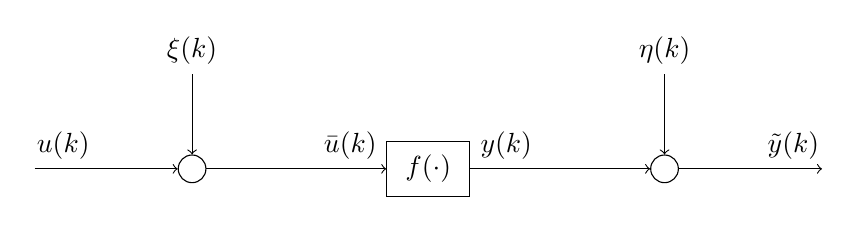
\begin{tikzpicture}[auto, node distance=2cm]

    % Block styles
    \tikzstyle{block} = [draw, rectangle, minimum height=2em, minimum width=3em]
    \tikzstyle{sum} = [draw, circle, inner sep=0pt, minimum size=1em]
    \tikzstyle{input} = [coordinate]
    \tikzstyle{output} = [coordinate]

    % Nodes
    \node [input] (input) {};
    \node [sum, right of=input, node distance=2cm] (sum1) {};
    \node [block, right of=sum1, node distance=3cm] (system) {$f(\cdot)$};
    \node [sum, right of=system, node distance=3cm] (sum2) {};
    \node [output, right of=sum2, node distance=2cm] (output) {};

    % Connections
    \draw [->] (input) -- node[pos=0.2] {$u(k)$} (sum1);
    \draw [->] (sum1) -- node[pos=0.8] {$\bar{u}(k)$} (system);
    \draw [->] (system) -- node[pos=0.2] {$y(k)$} (sum2);
    \draw [->] (sum2) -- node[pos=0.8] {$\tilde{y}(k)$} (output);
    
    % Noise terms
    \node [above of=sum1, node distance=1.5cm] (xi) {$\xi(k)$};
    \draw [->] (xi) -- (sum1);
    
    \node [above of=sum2, node distance=1.5cm] (eta) {$\eta(k)$};
    \draw [->] (eta) -- (sum2);

\end{tikzpicture}
\end{center}

\textit{Errors-in-variables} (EIV) problems refer to the most general case where both the input and the output collected samples are affected by noise.

\[
\xi = [\xi(1), \dots, \xi(H)] \in \mathcal{B}_{\xi}
\]
\[
\eta = [\eta(1), \dots, \eta(H)] \in \mathcal{B}_{\eta}
\]

$\mathcal{B}_{\xi}$ and $\mathcal{B}_{\eta}$ are bounded sets described by \textbf{\textit{polynomial constraints}.}

Most common case:
\[
\mathcal{B}_{\eta} = \left\{\eta : |\eta(k)| \leq \Delta_{\eta}\right\}, \quad \mathcal{B}_{\xi} = \left\{\xi : |\xi(k)| \leq \Delta_{\xi}\right\}
\]
which is a hyper-dimensional box.

A subset of this problem, as was discussed also in the previous chapter, is Output-Error, OE, set-up, meaning that the input signal is perfectly known.


\begin{center}    % Block styles
\begin{tikzpicture}[auto, node distance=2cm]

    \tikzstyle{block} = [draw, rectangle, minimum height=2em, minimum width=3em]
    \tikzstyle{sum} = [draw, circle, inner sep=0pt, minimum size=1em]
    \tikzstyle{input} = [coordinate]
    \tikzstyle{output} = [coordinate]

    % Nodes
    \node [input] (input) {};
    \node [block, right of=input, node distance=3cm] (system) {$f(\cdot)$};
    \node [sum, right of=system, node distance=3cm] (sum2) {};
    \node [output, right of=sum2, node distance=2cm] (output) {};

    % Connections
    \draw [->] (input) -- node[pos=0.5] {$u(k)$} (system);
    \draw [->] (system) -- node[pos=0.2] {$y(k)$} (sum2);
    \draw [->] (sum2) -- node[pos=0.8] {$\tilde{y}(k)$} (output);
    
    % Noise terms at the output
    \node [above of=sum2, node distance=1.5cm] (eta) {$\eta(k)$};
    \draw [->] (eta) -- (sum2);
\end{tikzpicture}
\end{center}\vspace{1cm}
where,
\begin{itemize}
\item 
\[
\eta = \left[\eta(1),\,\eta(2),\, \cdots,\,\eta(H)\right] \in \mathbb{B}_\eta
\]
\item \(\mathbb{B}_\eta\) is a bounded set described by \textbf{\textit{polynomial constraints}}.
\item Most common case: \(\mathbb{B}_\eta = \left\{\eta: \: |\eta(k)| \leq \Delta_\eta \right\}\)
\end{itemize}

The FPS for the general EIV problem is implicitly defined as follows:
\[
\begin{array}{c}
\mathbb{D}_\theta = \{ \theta \in \mathbb{R}^n : \, y(k) = f( y(k-1), y(k-2), \cdots, y(k-n),  u(k), u(k-1), \cdots \\[1ex]
, u(k-m), \theta_1, \theta_2, \cdots, \theta_{n+m+1}),k = n+1,\,n+2,\,\cdots,\,N,\: y(k) = \tilde{y}(k) - \eta(k), \\[1ex]
u(k) = \tilde{u}(k) - \xi(k),\: k=1,\,2,\,\cdots,\,N,\: |\xi(k)|\leq \Delta\xi(k),\: |\eta(k)\leq \Delta\eta(k),\: k = 1,\,2,\,\cdots,\,N \}
\end{array}
\]

The FPS for the case of \textbf{LTI descrete-time systems with EIV noise structure} is given by:
\[
\mathbb{D}_\theta = \left\{ \theta \in \mathbb{R}^p : \, (\tilde{y}(k) - \eta(k)) + \sum_{i=1}^{n} a_i (\tilde{y}(k - i) - \eta(k - i)) = \sum_{j=0}^{m} b_j (\tilde{u}(k - j) - \xi(k - j)), \right.
\]
\[
\left. t = n + 1, \dots, H, \quad |\xi(k)| \leq \Delta\xi(k), \quad |\eta(k)| \leq \Delta\eta(k), \quad k = 1, \dots, H \right\}
\]
This includes \(2N\) new variables involved in the FPS which are not variables in parameter space. Now, these variables should be eliminated, and this is not possible without setting some conservative conditions. \textbf{If you come up with an idea to do so without considering conservative conditions, you can publish a paper}. 

Since the FPS defined in the above equation depends on some additional unknownes( all the samples of the noise sequences). The constraints defining \(\mathbb{D}_\theta\) cannot be rearranged in such a way to eliminate dependancies on such additional variables. To solve the problem, we need to extend the space of decision variables in by defining the \textit{Extended Feasible Parameter Set}(EFPS).

\[
\begin{array}{c}
\mathcal{D}_{\theta,\eta,\xi} = \left\{ \theta \in \mathbb{R}^p, \eta \in \mathbb{R}^H, \xi \in \mathbb{R}^H : \right.
(y(k) - \eta(k) + \sum_{i=1}^{n} a_i ( y(k-i) - \eta(k-i)) = \\[2ex]
\sum_{j=0}^{m} b_j ( u(k-j) - \xi(k-j) ), \, t = n+1,\dots,H, \\[2ex]
|\xi(k)| \leq \Delta \xi(k), \, |\eta(k)| \leq \Delta \eta(k), \, k = 1,\dots,H \left.\right\}
\end{array}
\]
As you can see in the box below, here, we are expanding the space we are considering for FPS, hence EFPS.
\begin{align}
\fcolorbox{red}{white}{$\mathcal{D}_{\theta,\eta,\xi} = \left\{ \theta \in \mathbb{R}^p, \eta \in \mathbb{R}^H, \xi \in \mathbb{R}^H\right\}$}
\end{align}

A simplified graphical varsion is going to be like the following graph:

\begin{figure}[htbp]  % "h" for here, "t" for top, "b" for bottom, "p" for float page
    \centering
    \includegraphics[width=0.7\textwidth]{images/EFPS.png}
    \caption{A simplified, general graph of EFPS.}
    \label{fig:EFPS}
\end{figure}

In this case,
\[
\underline{\theta}_k = \min\limits_{\theta \in \mathbb{D}_\theta} \theta_k = \min\limits_{\theta, \eta, \xi \in \mathbb{D}_{\theta, \eta, \xi}} \theta_k
\]
That is,
\[
\begin{array}{rcl}
\theta_k & = & \min_{\theta \in \mathbb{D}_\theta, \eta, \xi} \theta_k \text{ subject to } \tilde{y}(k) - \eta(k) + \sum_{i=1}^{n} \theta_i(\tilde{y}(k-i) - \eta(k-i)) \\[1ex]
& = & \theta_{n+1}(\tilde{u}(k) - \xi(k)) + \sum_{j=1}^{m} \theta_{n+j+1}(\tilde{y}(k-j) - \xi(k-j)), \\[1ex]
& & \quad \forall k > n+1, \, |\xi(k)| \leq \Delta \xi, \, |\eta(k)| \leq \Delta \eta, \, \forall k
\end{array}
\]

The drawback is that EFPS is a non-convex set defined by \textbf{polynomial} (\textit{bilinear}) constraints.

\begin{factbox}[Professor's Quote:]
To the best of my knowledge, in the domain of non-convex functions, the only class that can be optimized up to the global minimum is the class of non-convex functions with polynomial constraints.
\end{factbox}

